\chapter{{Introduction}}
\label{chap:introduction}
\minitoc

\thispagestyle{empty}

\newpage
%%%%%%%%%%%%%%%%%%%%%%%%%%%%%%%%%%%%%%%%%%%%%%%%%%%%%%%%%%%%%%%%%%%%%%%%%%%%%%

%\section{Motivation}

%\clearpage

\section{Background}
\definecolor{brickred}{rgb}{0.8, 0.25, 0.33}
\lettrine[lines=4]{\color{brickred}M}{odelling} , analysis and control of \textit{nonsmooth} systems is an interesting and open problem which attracts the attention of a wide range of researchers, from physicists and mechanical engineers to specialists in control and automation~\citep{brogliato1999nonsmooth,stronge2018impact}.
The interaction between continuous and discrete-time dynamics arises, for instance, while considering the behavior of a mechanical system in presence of impacts: its dynamics cannot be represented only by means of differential equations. The theory of~\textit{hybrid dynamical systems} (HDS) is the formalism in which this type of models can be described. Overviews of this framework are given in~\citep{van2000introduction,haddad2006impulsive}. In particular, the most general and recent modeling approach is the one of \textit{hybrid inclusions} developed in recent years \citep{goebel2009hybrid}. This field of Automatic Controls generally investigates systems characterized by the interaction of continuous and discrete time dynamics as well as by multimodality \citep{Goebel2012}.
%
\newline

%
%%%%%%%%%%%%%%%%%%%%%%%%%%%%%%%%%%%%%%%%%%%%%%%%
%\subsection{The Manipulation Problem for Highly Dynamic Tasks}
%\subsection{The Role of Energy in Robot Control}
In the last three decades, the fundamental concept of \textit{energy} experienced an impressive growth process in engineering practice and in particular in system theory. 
%
%\newline
%
%
The framework of \textit{passivity--based control} (PBC) is now a well--established branch of nonlinear control theory and aims at treating dynamical systems as devices able to exchange energy, rather than to process signals \citep{ortega2001putting}. 
This is possible by equipping dynamical systems with additional structure (e.g. storage functions, supply rates, etc.) by means of which the concepts of energy and input/output characterization of the system are connected in a unique framework \citep{sontag2008input}.
%
\newline

%
In this context, another fundamental paradigm regards the \textit{interconnection} of systems by means of \textit{power ports} \citep{duindam2009modeling}, which led to the definition of \textit{port-Hamiltonian systems} \citep{MASCHKE1992359,ortega2001putting,van2014port}, the mathematical framework in which PBC developed naturally, merging geometry and network theory. Hence, the control problem reduces to the design of a dynamical system (the controller) and an interconnection structure that ``shapes'', in a desired way, the energy of the original system \citep{ortega2001putting,ortega2008control}.
%
%\newline
%
%
This approach allows control engineers to pay particular attention to the performance of the control system and not only to stabilizability (as common in nonlinear control).
%
%\newline
%
%
In classic robot control, the theory of passivity lead to several successful approaches, such as the \textit{gravity--compensation} \citep{arimoto1984stability} and \textit{impedance} controller \citep{secchi2007control}. Other interesting application are robots with flexible links \citep{macchelli2009} and elastic joints \citep{zhang2016}.
%
%%%%%%%%%%%%%%%%%%%%%%%%%%%%%%%%%%%%%%%%%%%%%%%%%%%%%%%
\subsection{Energy as Common Factor Among Interactions}\label{subsec:comm_fact}
%
Driven by a physical intuition, it is rather straightforward to recognize energy as the \textit{lingua franca} between different physical domains. This idea lead, in the early sixties, H. Paynter to establish the field of \textit{port--based modeling} \citep{paynter1961analysis}.
%
\newline

%
A physical system, in fact, may exhibit a \textit{dynamical behavior} if and only if some energy exchange happen within its \textit{internal structure} (components) or with the external world. In any physical domain there exists pair of dual variables (see Appendix A) often called \textit{flows} and \textit{efforts} which intrinsically form \textit{power ports}, interfaces through which energy flows \citep{secchi2007control}. Table \ref{tab:ef} lists the effort and flow variables for several physical domains.
%
\begin{table}[t]
	\centering
	\caption{Efforts and flows variables for various physical domains.}
	\begin{tabular}{|c|cc|cc|} \hline
			\rowcolor{gray!50}\textbf{Domain}&{\centering \textbf{Effort}}&&{\centering \textbf{Flow}}&\\\hline
			Mechanics (translational)&Force&$F$&Velocity&$v$\\\hline
			\rowcolor{gray!15}Mechanics (rotational)&Torque &$\tau$&Angular Velocity &$\omega$\\\hline
			Electric&Voltage &$v$&Current &$i$\\\hline
			\rowcolor{gray!15}Hydraulic&Pressure& $p$&Volume Flow &$Q$\\\hline
			Thermodynamic&Temperature &$T$&Entropy Flow &$\dot{E}$\\\hline
	\end{tabular}
	\label{tab:ef}
\end{table}
%
\newline

In robot manipulation, this description of dynamical phenomena may result particularly useful to model the interaction between the robot end--effector and the object, which indeed exchange energy with each other in a continuous fashion.
%
In fact, the port--Hamiltonian framework allows to explicitly capture the physical phenomena behind this continuous interaction. Furthermore, in this perspective, the robot controller can also be thought as an other dynamical system interconnected with the robot and exchanging energy with it. 
This approach results to be both, general and versatile.
%
The theory of passivity--based control of port--Hamiltonian system has been already successfully applied in a variety of manipulation tasks: from grasping \citep{stramigioli99} and soft--finger manipulation \citep{ficuciello2010} to non--prehensile tasks, e.g. object rolling \citep{donaire2017,serra2019}.
%
\newline

%
Besides, when the robot tasks involve \textit{nonsmooth} phenomena such as mechanical impacts or dynamic friction \citep{brogliato1999nonsmooth}, the classical passivity--based techniques cease to work due to the discontinuities in system's state along trajectories. 

However it can be noticed that energy is the undisputed protagonist also of this type on discrete (instantaneous) interactions. Thus, an energy--based reasoning might be carried out to overcome the challenges given by the hybrid nature of these robot tasks.  

From now on, we will refer to any robotic tasks which is hybrid in nature, i.e. it includes interacting continuous and discrete phenomena, as \textit{highly dynamic tasks}.
%%%%%%%%%%%%%%%%%%%%%%%%%%%%%%%%%%%%%%%%%%%%%%%%%%%%%%%%%%%%%%%%%%%%%
%\subsection{Hybrid port--Hamiltonian System: a New Tool For Robotics}
\subsection{Research Problem: Control Highly Dynamic Robotic Tasks}
%
The extension of passivity--based control of port--Hamiltonian systems to the hybrid case is highly desirable. In fact, this will allow to establish a new general and unified framework to model and control robots performing highly dynamic tasks.
%
\newline

%
Examples of these tasks in the manipulation context are:
ball--juggling \citep{sanfelice2007hybrid, tian2013}, ball--dribbling \citep{Batz2010, haddadin2018exploiting} or even tossing/catching of a deformable object \citep{ruggero2018}. 
Other hybrid tasks may be related to \textit{self manipulation}, e.g. dynamic walking \citep{spong2007,westervelt2018feedback}, hopping robots \citep{Ishikawa2003} and control of powered exoskeletons \citep{harib2018feedback,lv2018design}. The one--dimensional version of the ball--juggling and ball--dribbling systems are represented in Fig. \ref{fig:1D}.
%
\newline

%
One of the most clear proofs of the necessity of an novel unified framework merging energy--based approaches to hybrid systems is given by all the research work present in literature: although they belong to the same class of robot control problems, each tasks is solved with \textit{ad--hoc} solutions, without any analysis of a bigger picture.  
%
\newline

Furthermore, as underlined in Subsection \ref{subsec:comm_fact}, the span of validity of this new general framework could indeed be extended to any physical domain, and thus employed to find potential solutions in different branches of engineering.
%
\begin{figure}[!t]
	\centering
	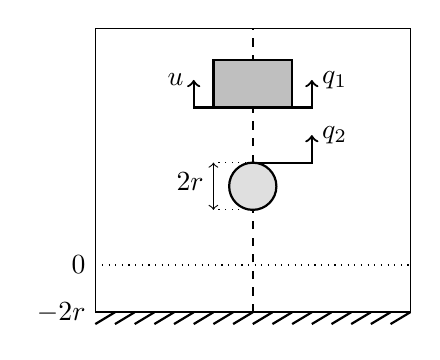
\begin{tikzpicture}
	%
	% axes
	\draw[thick] (0,-0.6)--(4,-0.6);
	\draw[dotted] (0,0) node[anchor = east] {\color{black}$0$}--(4,0);
	\draw[thick,dashed] (2,-0.6) -- (2,3);
	\draw (0,-0.6) node[anchor = east] {$-2r$} -- (4,-0.6) -- (4,3) -- (0,3) -- (0,-0.6);
	
	% robot
	\fill[gray!50, draw = black,thick] (1.5,2) rectangle (2.5,2.6);
	% ball
	\fill[gray!25, draw=black,thick] (2,1) circle (0.3);
	%	
	\draw[thick,->] (2.5,2) -- (2.75,2) -- (2.75,2.35) node[anchor=west] {$q_1$};
	\draw[thick,->] (1.5,2) -- (1.25,2) -- (1.25,2.35) node[anchor=east] {$u$};
	\draw[thick,->] (2,1.3) -- (2.75,1.3) -- (2.75,1.65) node[anchor=west] {$q_2$};
	%
	\draw[dotted] (2,1.3) -- (1.5,1.3);
	\draw[dotted] (2,0.7) -- (1.5,0.7);
	\draw[<->] (1.5,0.7) -- (1.5,1.3)  node[anchor=north east] {$2r$};
	%
	\foreach \x in {0,0.25,0.5,0.75,1,1.25,1.5,1.75,2,2.25,2.5,2.75,3,3.25,3.5,3.75}
	\draw[thick] (\x,-0.75) -- (\x+0.25,-0.6);
\end{tikzpicture}
	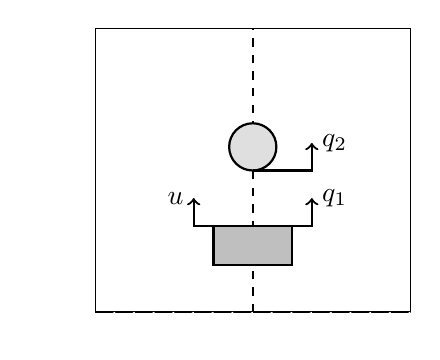
\begin{tikzpicture}
	%
	\draw[thick] (0,-0.6)--(4,-0.6);
	\draw[thick,dashed] (2,-0.6) -- (2,3);
	\draw (0,-0.6)  node[anchor = east] {\color{white}$-2r$} -- (4,-0.6) -- (4,3) -- (0,3) -- (0,-0.6);
	
	% robot
	\fill[gray!50, draw = black,thick] (1.5,0) rectangle (2.5,0.5);
	% ball
	\fill[gray!25, draw=black,thick] (2,1.5) circle (0.3);
	%	
	\draw[thick,->] (2.5,0.5) -- (2.75,0.5) -- (2.75,0.85) node[anchor=west] {$q_1$};
	\draw[thick,->] (1.5,0.5) -- (1.25,0.5) -- (1.25,0.85) node[anchor=east] {$u$};
	\draw[thick,->] (2,1.2) -- (2.75,1.2) -- (2.75,1.55) node[anchor=west] {$q_2$};
	\foreach \x in {0,0.25,0.5,0.75,1,1.25,1.5,1.75,2,2.25,2.5,2.75,3,3.25,3.5,3.75}
	\draw[color = white] (\x,-0.755) -- (\x+0.25,-0.6);
\end{tikzpicture}
	\caption[One--dimensional ball--dribbling and ball--juggling robotic systems.]{One--dimensional ball--dribbling (left) and ball--juggling (right) robotic systems. The position of the robot (rectangle), is represented by the variable $q_1$ while $u$ is an input force applied to it. The position of the ball (circle), of radius $r$, is represented by $q_2$. The ball--juggling system presents a single impact, i.e. the one between the robot and the ball. The ball--dribbling system, instead, is characterized by two impacts: ball--robot and ball--ground.}
	\label{fig:1D}
	%
\end{figure}
%
%%%%%%%%%%%%%%%%%%%%%%%%%%%%%%%%%%
\subsection{Beyond Robot Control}
It has been proven that a novel unified framework for controlling highly dynamic robotic tasks is needed but cannot be approached in a systematic general way due to the \textit{nonsmooth} nature of the robotic tasks.
%
\newline

%
However, many control systems presents discontinuities and multimodality due to the control algorithm itself rather then physics. 
For example, a system subjected to a \textit{sliding--mode controller} \citep{pisano2011sliding} is, technically speaking, an hybrid system. Moreover, the whole framework of \textit{switching control} belongs to field of hybrid dynamical systems.
%
\newline

%
Very simple practical example of how a controller give an hybrid nature to dynamical systems, are the temperature regulator of a room or the water--level control in tanks.
%
\newline
    
%
In the light of this considerations, it is legitimate pose the following questions: \newline
\textit{Can hybrid control systems be modeled from an energetic point of view in port--Hamiltonian fashion?}\newline
\textit{If yes, which theoretical advantages would this formulation give?}

%%%%%%%%%%%%%%%%%%%%%%%%%%%%%%%%%%%%%%%
\subsection{The Identification Problem}
%
As common in Automatic Controls, controller design, simulations and diagnostics of hybrid dynamical systems require an accurate knowledge of the model. However, these {processes} are always characterized by sets of parameters which are typically not available.
%
\newline

%
System identification techniques are the interface between real world application and mathematical world of control theory and mathematical abstraction~\citep{LJUNG20101}. These methods aim to obtain estimates of the parameters and update the model from direct measurements collected during the time evolution of the system~\citep{soderstrom2018errors,SODERSTROM2019}.
%
\newline

%
Dealing with robotic systems, it is well known that inertial parameters must often be thoroughly estimated with well designed identification experiments. Moreover, if the robot experiences impacts or sudden state changes, it is intuitive to understand that further parameters given by the hybrid part of the system must also be estimated. 
Thus, in order to implement any robot controllers for highly dynamic tasks, it is necessary to solve the identification problem first.
%
\newline

%
The majority of the literature on identification of hybrid systems is related to classes of (discrete--time) Piece Wise Affine systems (PWA), i.e. systems which are defined by subdividing the  space into polyhedral regions which have associated an affine state update equation \citep{Bemporad,Ferrari,Juloski,juloski2005bayesian,Paoletti}.
% 
\newline

%
Besides, the identification of hybrid dynamical system in the form of \textit{hybrid inclusions} has to be explored yet. In fact, a systematic identification procedure for this class of systems currently is still missing. Note that, many of the robotics tasks discussed above can be modeled within this framework.
%
\newline

%
Real implementation of those tasks would undoubtedly require the knowledge of some parameters of the plant. Thus, if a novel unified modeling framework merging port--Hamiltonian and hybrid systems is proposed alongside new control techniques, the systematic estimation of physical parameters of both continuous (e.g. mass, inertia, friction) and discrete (e.g. impact restitution coefficient) parts of models  will be needed.
%
\clearpage
%%%%%%%%%%%%%%%%%%%%%%%%%%%%%%%%%%%%%%%%%%%%%%%%%%%%%%%%%%%%%%%%%%%%%%%%%%%%%%%

\section{{Aims and Objectives}}\label{sec:aim}
The aim of this thesis is to present a novel control theoretical framework for physical systems with nonsmooth and multimodal behaviors, with a special insight toward robot control tasks where the current--state--of--the--art approaches fail.

The main objectives are:
%
\begin{itemize}
    \item [1.] \textbf{to develop a novel control theoretical framework by merging the theories of port--Hamiltonian systems and hybrid systems}.
    
    With the aim of solving a robot control problem, the theory of \textit{hybrid port--Hamiltonian systems} is developed combining the theories of port--Hamiltonian systems and \textit{hybrid inclusions}, one of the most general representations of hybrid dynamical systems.
    \newline
    %
    \item [2.] \textbf{to apply the developed theory to a robot control task and prove its effective within the robotics framework}. 
    
    Considering the ball--dribbling robot problem, a novel controller, the \textit{iterative energy shaping} is systematically synthesized, proving the capabilities of the proposed framework.
    \newline
    %
    \item [3.] \textbf{to demonstrate how the developed theory goes beyond robotics and can be used to model a broad variety of control systems}. 
    
    A novel nonlinear hybrid controller for linear time--invariant system is derived from passivity--based techniques, and then this purely control theoretical problem is expressed via hybrid port--Hamiltonian systems.
    \newline
    %
    \item[4.] \textbf{to derive a new systematic identification procedure for a class of hybrid systems}.
    
    As most of hybrid control systems (including the proposed ones) require some knowledge of the physical parameters of the controlled plant, a new systematic procedure is presented to solve the estimation problem. This method can be applied to a variety of hybrid port--Hamiltonian systems 
    
    \end{itemize}
%





%
\clearpage
%%%%%%%%%%%%%%%%%%%%%%%%%%%%%%%%%%%%%%%%%%%%%%%%%%%%%%%%%%%%%%%%%%%%%%%%%%%%%%%

\section{Thesis Content and Structure}
\subsection{Thesis Outline}
This thesis is structured in seven chapters which implement the aim described in \ref{sec:aim}. 
These seven chapter can be logically clustered in four main parts: Introduction and background, theoretical results, applications and conclusions. In line with the objectives, a detailed structure of this thesis is shown in Figure \ref{fig:ThesisStructure}.
%
\newline

%
\textbf{Chapter 1} describes the main motivations, purpose and approach of this study.
%
\newline

%
\textbf{Chapter 2} briefly introduces the fields of port--Hamiltonian systems and hybrid dynamical systems. Throughout the chapter, several illustrative examples related to robotics, mathematical biology and physics are provided to highlight the practical importance of the presented theoretical concepts. 

In the first half of the chapter, the input--state--output model of a port-Hamiltonian system is derived and its most relevant properties are described. Moreover, the basic theory of the energy--balancing passivity--based control is also presented. In the second part of the chapter, the basic results on hybrid systems are introduced. In particular, it will be focused on the class of \textit{hybrid inclusions} and its stability/passivity theory.  The chapter concludes with a summary of the previous attempts to merge the two frameworks and their main limitations. 
%
\newline

%
\textbf{Chapter 3} deals with the definition and characterization of hybrid-port Hamiltonian systems. Starting from the concepts revised in the previous chapter, the new framework is here consistently developed. First, the basic assumptions are stated and the hybrid port--Hamiltonian model is derived. The concept of passivity is subsequently extended to the new model. Necessary and sufficient conditions for passivity are also reported and proved. Then, Lyapunov stability is extended from the one for hybrid inclusions. Finally, all the previous results are used to transfer to the hybrid case some of the features of passivity--based control for port--Hamiltonian systems. As for Chapter 2, application examples will be provided throughout the chapter.
%
\newline

%
\textbf{Chapter 4} introduces the first real application of the developed theory. In particular, the problem of modeling and control a ball--dribbling robot is considered. The main challenges offered by this systems are: under-actuation, dynamic decoupling between the robot and the ball and impacting interactions. First, the system is consistently modeled in hybrid port--Hamiltonian form. Then, a novel energy--based controller is derived from physical intuitions on the system. This controller enhance the classic energy shaping with the iterative learning, allowing the robot to rhythmically bounce the ball at a desired height. Simulations are performed to prove the effectiveness and robustness of the controller.   
%
\newline

%
\textbf{Chapter 5} considers the problem of controlling a linear time--invariant system with a finite number of set points. At first, a nonlinear passive controller is used to stabilize simultaneously all the desired set points. Then, a hybrid optimal impulse controller is designed to switch the between the set points. Numerical simulations are carried out for a mechanical system, proving the results. Alongside the theoretical relevance of the developed control technique, it is finally shown how the controlled system can be modeled as hybrid port--Hamiltonian system, implicitly inheriting some useful properties to analyze its behaviour.
%
\newline

%
\textbf{Chapter 6} proposes a new systematic approach for the identification of a class of hybrid dynamical systems. The main challenge offered by the considered class of systems is the detection of state discontinuities from a time series of state measurements. The proposed solution is based on the analytical computation of an upper bound on the numerically computed time--derivative of the state, above which the system is considered to be ``jumping''. After implementing the jump detection function, the parameters of the system are estimated recursively. Simulations are performed on a mechanical systems to show the effectiveness of the proposed method.
\newline

%
\textbf{Chapter 7} presents the conclusions of this study and future work.
%
\begin{figure}[b]
    \centering
    \definecolor{darkspringgreen}{rgb}{0.09, 0.45, 0.27}
    \tikzstyle{container} = [rectangle, draw, semithick, rounded corners,
                     text width=44mm, minimum height=11mm, align=center,
                     fill=white, drop shadow, inner sep=0.6cm]
    \begin{tikzpicture}[
        node distance = 5mm and 4mm,
        %every node/.style = {font=\bfseries\itshape},
        chapter/.style = {rectangle, draw, semithick, rounded corners,
                     text width=44mm, minimum height=9mm, align=center,
                     fill=white, drop shadow},  
                     ys/.style = {yshift=-5mm}         
                    ]
        \draw[thick] (0,0)  coordinate (A1)
                    node[below right] {Preliminaries \& Background} 
                    -- + (\textwidth,0)
                    coordinate (B1);
        \node (ch1) [chapter, below=of $(A1)!0.5!(B1)$]         {\textbf{Chapter 1}\\ \textit{Introduction}};
        \node (ch2a) [chapter, below  left=1.5cm and -2cm of ch1] {Port--Hamiltonian Systems};
        \node (ch2b) [chapter, below right=1.5cm and -2cm of ch1] {Hybrid Dynamical Systems};
        \node [container,fit=(ch2a) (ch2b), yshift = 0.5cm] (c1) {\textbf{Chapter 2}\\ \textit{Preliminaries}\textcolor{white}{\\aa\\aa}};
        \node (ch2a) [chapter, below  left=1.5cm and -2cm of ch1] {Port--Hamiltonian Systems};
        \node (ch2b) [chapter, below right=1.5cm and -2cm of ch1] {Hybrid Dynamical Systems};
        %
        \draw[thick] ([ys] A1 |- ch2a.south)  coordinate (A2)
                    node[below right] {Theoretical Results}
                    -- + (\textwidth,0)
                    coordinate (B2);
        \node (ch3) [chapter, below=of $(A2)!0.5!(B2)$,text width=54mm, fill = gray!50]   {\textbf{Chapter 3}\\\textit{Hybrid Port--Hamiltonian Systems}};
        %\node (ch3) [chapter, below  left=of $(A2)!0.5!(B2)$]   {State of the Art};
        %\node (ch4) [chapter, below right=of $(A2)!0.5!(B2)$]   {Building of Theory};
        \draw[thick] ([ys] A1 |- ch3.south)  coordinate (A3)
                    node[below right] {Applications}
                    -- + (\textwidth,0)
                    coordinate (B3);
        \node (ch4) [chapter, below=of $(A3)!0.5!(B3)$,text width=84mm, fill = gray!50] {\textbf{Chapter 4}\\\textit{Iterative Energy shaping of a Ball--dribbling Robot}};
        \node (ch5) [chapter, below=of ch4,text width=84mm, fill = gray!50]                     {\textbf{Chapter 5}\\\textit{Multistable Energy Shaping with Hybrid Mode Selector}};
        \node (ch6) [chapter, below=of ch5,text width=84mm, fill = gray!50]                     {\textbf{Chapter 6}\\\textit{Identification of a Class of Hybrid Systems}};
        \draw[thick] ([ys] A1 |- ch6.south)  coordinate (A4)
                    node[below right] {Conclusion}
                    -- + (\textwidth,0)
                    coordinate (B4);
        \node (ch7) [chapter, below=of $(A4)!0.5!(B4)$]         {\textbf{Chapter 7}\\Discussion and conclusions};
        %\node (ap1) [chapter, below  left=of ch7]               {\textbf{Appendix A}};
        %\node (ap2) [chapter, below =of ch7]                    {\textbf{Appendix B}};
        %\node (ap3) [chapter, below right=of ch7]               {\textbf{Appendix C}};
        %
        \draw [-latex, ultra thick, blue] (ch1)--(c1);
        \draw [-latex, ultra thick, blue] (ch2a.south) to[out=-45,in=90] (ch3.north);
        \draw [-latex, ultra thick, blue] (ch2b.south) to[out=-135,in=90] (ch3.north);
        \draw [-latex, ultra thick, blue] (ch3.south) to[out=-90, in=90] (ch4.north);
        \draw [-latex, ultra thick, blue] (ch3.south) to[out=-155,in=130,distance=3.5cm] (ch5.west);
        \draw [-latex, ultra thick, red] (ch2b.south) to[out=-45,in=30,distance=2.5cm] (ch6.east);
        \draw [-latex, ultra thick, darkspringgreen] (ch6.south)--(ch7.north);
        \draw [-latex, ultra thick, darkspringgreen] (ch5.west) to[out=200,in=180,distance=1.5cm] (ch7.west);
        \draw [-latex, ultra thick, darkspringgreen] (ch4.west) to[out=200,in=180,distance=3cm] (ch7.west);
    \end{tikzpicture}
    \vspace{5mm}
    \caption[Thesis outline.]{Thesis outline. The coloured arrows indicate the logical flows of the contents throughout the thesis, highlighting, e.g., how the theory presented in the first chapters is employed in the various applications. Chapters in light gray blocks contain exclusively original content developed by the author,}
    \label{fig:ThesisStructure}
\end{figure}
%
%\newline
%
%
\subsection{Thesis Content}
This thesis is developed across three main broad fundamental fields: control theory, robotics and statistics. The Venn diagram in Fig. \ref{fig:venn} clarifies how the contents are interconnected within the main research fields. In particular, the first three chapters are related to pure control as port--Hamiltonian systems and hybrid dynamical systems are firstly introduced in Chapter 2 and then merged in Chapter 3. Chapter 5 is also mostly related to theoretical aspects. However, the concepts of Chapter 4, which introduces the ball--dribbling robot encompasses the intersection of control theory and robotics with . Chapter 6 treats the parameters estimation problem for a class of hybrid dynamical systems, spanning in the intersection of control theory and statistics.

\begin{figure}
    \centering
    \def\firstcircle{(0,0) circle (2.5cm)}
    \def\secondcircle{(45:3.5cm) circle (2.5cm)}
    \def\thirdcircle{(0:4.5cm) circle (2.5cm)}
    \def\id{(3,-2.5) ellipse (0.65 and 0.65)}
    \def\hds{(3,-1.3) ellipse (1.5 and 1.2)}
    \def\ph{(3.2,0) ellipse (1.5 and 1.2)}
    \definecolor{carminered}{rgb}{1.0, 0.0, 0.22}
    \definecolor{cerulean}{rgb}{0.0, 0.48, 0.65}
    \definecolor{bluegray}{rgb}{0.4, 0.6, 0.8}
    \definecolor{amber}{rgb}{1.0, 0.75, 0.0}
    \definecolor{emerald}{rgb}{0.31, 0.78, 0.47}
    %
    \begin{tikzpicture}
        \draw[thick, fill=gray!30,fill opacity=0.3] \firstcircle;
        \draw[thick, fill=gray!30,fill opacity=0.3] \secondcircle node [above] {};%{\small Control Theory};
        \draw[thick, fill=gray!30,fill opacity=0.3] \thirdcircle node [below] {};%{Statistics};
        \draw[thick, fill=gray!50,fill opacity=0.4, rotate = 60] \hds node [below] {};%{Statistics};
        \draw[thick, fill=gray!50,fill opacity=0.4, rotate = 60] \ph node [below] {};%{Statistics};
        \draw[thick, fill=gray!50,fill opacity=0.4, rotate = 60] \id node [below] {};%{Statistics};
        %
        \begin{scope}[rotate = 60]
            \clip \hds;
            \draw[thick, fill = amber] \ph;
        \end{scope}
        %
        \begin{scope}[rotate = 60]
            \clip \hds;
            \clip \firstcircle;
            \draw[-,black,thick, fill = bluegray] \ph;
        \end{scope}
        %
        \begin{scope}[rotate = 60]
            \clip \hds;
            \fill[emerald] \id;
        \end{scope}
        %%%%%%%%%%%%
        \draw (0,0)   node[]{\textbf{Robotics}};
        \draw (0:4.5) node[]{\textbf{Statistics}};
        \draw (2.55,4.45) node[]{\textbf{Control Theory}};
        \draw (-1,4.75) node[] (ph) {Port--Hamiltonian Systems};
        \draw (7.25,3.25) node[] (hds) {Hybrid Dynamical Systems};
        \draw (8,2) node[] (id) {System Identification};
        %
        \draw[-o, thick] (ph.south) to[out = -90,in = 150] (1.5,3);
        \draw[-o, thick] (hds.south) to[out = -90,in = 50] (3.5,2.5);
        \draw[-o, thick] (id.south) to[out = -90,in = -50] (3.85,1.25);
        %%%
        \draw (-1,-3) node[] (ch4) {\color{amber}\textbf{Chapter 4}};
        \draw (3,-3) node[] (ch5) {\color{bluegray}\textbf{Chapter 5}};
        \draw (7,-3) node[] (ch6) {\color{emerald}\textbf{Chapter 6}};
        %
        \draw[-o, dashed, thick] (ch4.north) to[out = 45,in = 180, distance = 4cm] (2.35,2.5);
        \draw[-o, dashed, thick] (ch5.north) to[out = 110,in = 250] (1.6,1.75);
        \draw[-o, dashed, thick] (ch6.north) to[out = 120,in = 250, distance = 3cm] (3.4,1.5);
    \end{tikzpicture}
    \vspace{5mm}
    \caption[Venn diagram of the contents presented in this thesis.]{Venn diagram of the contents presented in this thesis. In particular, Chapters 3 and 5 are related to theoretical aspects of hybrid port--Hamiltonian systems. Chapter 4 presents the application of hybrid port--Hamiltonian systems to robotics. Finally, Chapter 6 deals with the identification of hybrid systems, located in the meeting point of control theory and statistics.}
    \label{fig:venn}
\end{figure}

\clearpage
%%%%%%%%%%%%%%%%%%%%%%%%%%%%%%%%%%%%%%%%%%%%%%%%%%%%%%%%%%%%%%%%%%%%%%%%%%%%%%%
